\documentclass[11pt,a4paper]{article}

% ======================================================================
% College Assistant -- Software Copyright / Source Code Submission
% Statement of Particulars (India) + Source Code Excerpts + Declaration
% + Proprietary Software Licence, combined into a single document.
% ======================================================================

\usepackage[margin=1in]{geometry}
\usepackage{fontspec}
\setmainfont{Latin Modern Roman}
\newfontfamily\monofont{Latin Modern Mono}
\usepackage{titlesec}
\usepackage{enumitem}
\usepackage{fancyhdr}
\usepackage{xcolor}
\usepackage{hyperref}
\usepackage{tabularx}
\usepackage{longtable}
\usepackage{tikz}
\usetikzlibrary{positioning,fit,shapes.geometric}
\usepackage{listings}
\usepackage{needspace}
\usepackage{xurl}
\urlstyle{tt}

\definecolor{hdrnavy}{RGB}{31,55,86}
\definecolor{hdrblue}{RGB}{224,232,242}
\definecolor{rulegray}{RGB}{120,120,120}

\hypersetup{
    colorlinks=true,
    linkcolor=black,
    urlcolor=blue,
    pdftitle={College Assistant -- Software Copyright Source Code Submission},
    pdfauthor={Vikas Bhowate, Om Gawande, Yash Garad, Harshal Ninawe, Aanchal Kalambe, Aditi Parshivanikar},
    pdfsubject={Software Copyright Source Code Submission and Proprietary Licence}
}

\titleformat{\section}{\large\bfseries}{\thesection.}{0.6em}{}
\titleformat{\subsection}{\normalsize\bfseries}{\thesubsection}{0.6em}{}
\titlespacing*{\section}{0pt}{1.4em}{0.6em}

\setlength{\headheight}{14pt}
\pagestyle{fancy}
\fancyhf{}
\fancyhead[L]{College Assistant -- Software Copyright Source Code Submission}
\fancyhead[R]{\thepage}
\renewcommand{\headrulewidth}{0.4pt}

\setlist[enumerate,1]{label=(\alph*)}

% ---- code-listing style -------------------------------------------------
\lstdefinestyle{submission}{
    basicstyle=\monofont\scriptsize,
    numbers=left,
    numberstyle=\tiny\color{gray},
    numbersep=8pt,
    breaklines=true,
    breakatwhitespace=false,
    showstringspaces=false,
    tabsize=4,
    frame=single,
    rulecolor=\color{rulegray},
    framesep=4pt,
    columns=flexible,
    keepspaces=true,
    upquote=true,
    literate={—}{{---}}1 {…}{{\ldots}}1
}
\lstset{style=submission}

\newcommand{\FileHeader}[4]{%
  \begin{center}
  \renewcommand{\arraystretch}{1.3}
  \begin{tabularx}{\linewidth}{|>{\bfseries}l X|>{\bfseries}l X|}
    \hline
    \rowcolor{hdrblue}
    File Name: & #1 & Language: & #2 \\
    \hline
    \rowcolor{hdrblue}
    Module: & #3 & Lines: & #4 \\
    \hline
  \end{tabularx}
  \end{center}
  \vspace{-0.3em}
}
\usepackage{colortbl}

\newcommand{\OwnerName}{Dr Vikas Bhowate}
\newcommand{\OwnerEmail}{vipbhowate@gmail.com}
\newcommand{\SoftwareName}{College Assistant}
\newcommand{\SoftwareTagline}{A Multi-Agent Retrieval-Augmented Question Answering System}
\newcommand{\CopyrightYear}{2026}

\begin{document}

% =====================================================================
% PAGE 1 -- TITLE / STATEMENT OF PARTICULARS
% =====================================================================
\begin{center}
    {\LARGE \bfseries Software Copyright}\\[0.3em]
    {\LARGE \bfseries Source Code Submission}\\[1em]
    {\large Statement of Particulars --- Computer Programme (India)}
\end{center}

\vspace{1.2em}

\renewcommand{\arraystretch}{1.5}
\begin{tabularx}{\linewidth}{|>{\bfseries}p{4cm}|X|}
\hline
Project Title & \SoftwareName\ --- \SoftwareTagline \\
\hline
Version & 1.0 \\
\hline
Author(s) &
Dr Vikas Bhowate (Project Guide) \newline
Mr Om Gawande \newline
Mr Yash Garad \newline
Mr Harshal Ninawe \newline
Ms Aanchal Kalambe \newline
Ms Aditi Parshivanikar \\
\hline
Applicant / Owner & \OwnerName \\
\hline
Programming Languages & Python (Django / Django REST Framework), JavaScript (React), SQL \\
\hline
Frameworks \& Services & Django, Django REST Framework, React, Vite, Tailwind CSS, PostgreSQL, Qdrant, Ollama (local LLM inference), Caddy \\
\hline
Date of Creation & 2026 \\
\hline
Nature of Work & Original literary work --- Computer Programme (Source Code) \\
\hline
\end{tabularx}

\vfill
\begin{center}
\small\itshape This document combines the Statement of Particulars, source-code
excerpts and declaration prepared for copyright registration with the
project's proprietary software licence, into a single reference file.
\end{center}

\newpage

% =====================================================================
% SOFTWARE DESCRIPTION
% =====================================================================
\section*{Software Description}

\SoftwareName\ is an offline, self-hosted AI assistant that answers
questions about a college's database --- courses, departments, faculty,
fees, schedules, and more --- through a simple chat website. It combines a
React/Vite web client with a Python (Django REST Framework) backend. A
multi-agent pipeline routes each question to a SQL agent for structured
records, a retrieval-augmented-generation (RAG) agent for descriptive
search over a vector store, and an optional web agent for official college
pages; a synthesis agent then composes the final answer. All language-model
inference runs locally via Ollama, so no student or institutional data
leaves the server.

The software is organised into the following major modules:

\renewcommand{\arraystretch}{1.3}
\begin{tabularx}{\linewidth}{|>{\bfseries}p{3.9cm}|X|}
\hline
Authentication \& Accounts & Staff/user authentication, password hashing,
JWT session issuance, and request throttling
(\texttt{accounts/views.py}, \texttt{accounts/permissions.py},
\texttt{accounts/throttling.py}). \\
\hline
Orchestrator & Core request pipeline that routes each question across the
agents below, merges their output, and applies caching and concurrency
control (\texttt{orchestrator/service.py}, \texttt{orchestrator/views.py},
\texttt{orchestrator/cache.py}). \\
\hline
Router Agent & Classifies each incoming question via a local LLM to decide
whether it needs the SQL agent, the RAG agent, or both
(\texttt{router\_agent/classifier.py}, \texttt{router\_agent/llm\_client.py}). \\
\hline
SQL Agent & Generates and safely executes read-only SQL against the college
database behind a query guard and schema allow-list
(\texttt{sql\_agent/service.py}, \texttt{sql\_agent/guard.py},
\texttt{sql\_agent/schema.py}). \\
\hline
RAG Agent & Embeds each question and retrieves descriptive context from the
Qdrant vector store (\texttt{rag\_agent/service.py},
\texttt{rag\_agent/vector\_store.py}, \texttt{rag\_agent/embedder.py}). \\
\hline
Synthesis Agent & Composes the final natural-language answer, streaming or
otherwise, from the retrieved SQL/RAG/web context via a local LLM
(\texttt{synthesis\_agent/service.py}, \texttt{synthesis\_agent/llm\_client.py}). \\
\hline
Web \& Verification Agents & Fetches and summarises official college web
pages when configured, and cross-checks generated answers before they are
returned (\texttt{web\_agent/service.py}, \texttt{orchestrator/verification.py}). \\
\hline
Audit \& Health & Request/action logging and health-check endpoints for
each downstream dependency (\texttt{audit/models.py}, \texttt{health/views.py}). \\
\hline
Sync Worker & Background service that watches the college database's
change queue, converts changed rows to text, generates embeddings, and
upserts them into Qdrant (\texttt{sync\_worker/}). \\
\hline
Frontend & React/Vite chat client with markdown rendering, authentication
screens, sidebar, and streaming chat UI
(\texttt{frontend/src/App.jsx}, \texttt{components/Chat.jsx},
\texttt{components/Login.jsx}). \\
\hline
\end{tabularx}

\newpage

% =====================================================================
% SYSTEM ARCHITECTURE
% =====================================================================
\section*{System Architecture}

The following diagram depicts the layered system architecture of the
\SoftwareName\ platform, spanning the client, API, backend agent, external
service, and data layers.

\begin{center}
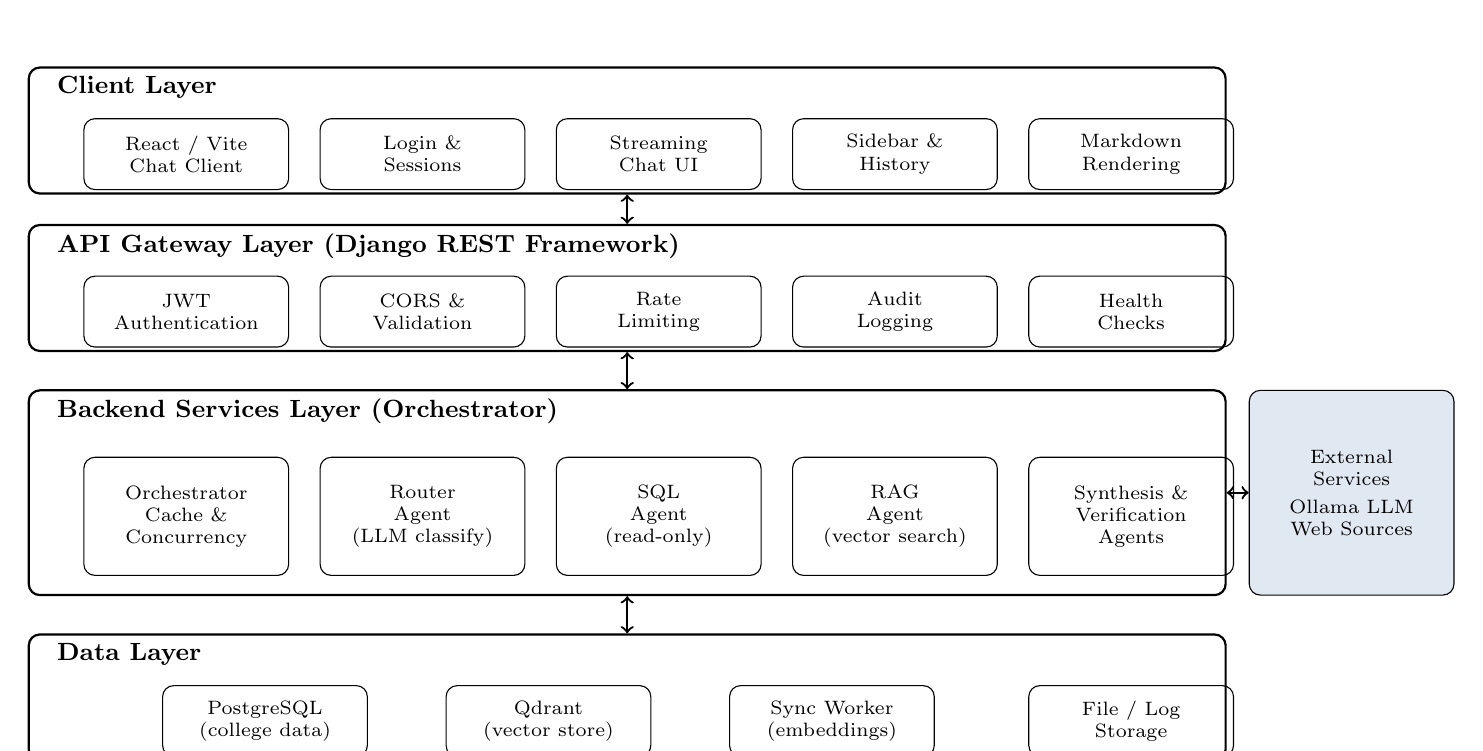
\begin{tikzpicture}[
  layer/.style={draw, rounded corners, thick, minimum width=15.2cm, align=center, font=\bfseries\small},
  box/.style={draw, rounded corners, minimum width=2.6cm, minimum height=0.9cm, align=center, font=\scriptsize},
  extbox/.style={draw, rounded corners, minimum width=2.6cm, minimum height=0.9cm, align=center, font=\scriptsize, fill=hdrblue},
  every node/.style={font=\scriptsize}
]

% Client layer
\node[layer, minimum height=1.6cm] (client) at (0,9.6) {};
\node[anchor=north west, font=\bfseries\small] at (client.north west) {\ \ Client Layer};
\node[box] (webclient) at (-5.6,9.3) {React / Vite\\Chat Client};
\node[box] (login) at (-2.6,9.3) {Login \&\\Sessions};
\node[box] (chatui) at (0.4,9.3) {Streaming\\Chat UI};
\node[box] (sidebar) at (3.4,9.3) {Sidebar \&\\History};
\node[box] (markdown) at (6.4,9.3) {Markdown\\Rendering};

% API layer
\node[layer, minimum height=1.6cm] (api) at (0,7.6) {};
\node[anchor=north west, font=\bfseries\small] at (api.north west) {\ \ API Gateway Layer (Django REST Framework)};
\node[box] (jwt) at (-5.6,7.3) {JWT\\Authentication};
\node[box] (cors) at (-2.6,7.3) {CORS \&\\Validation};
\node[box] (throttle) at (0.4,7.3) {Rate\\Limiting};
\node[box] (audit) at (3.4,7.3) {Audit\\Logging};
\node[box] (health) at (6.4,7.3) {Health\\Checks};

% Backend services layer
\node[layer, minimum height=2.6cm] (backend) at (0,5) {};
\node[anchor=north west, font=\bfseries\small] at (backend.north west) {\ \ Backend Services Layer (Orchestrator)};
\node[box, minimum height=1.5cm] (orch) at (-5.6,4.7) {Orchestrator\\Cache \&\\Concurrency};
\node[box, minimum height=1.5cm] (router) at (-2.6,4.7) {Router\\Agent\\(LLM classify)};
\node[box, minimum height=1.5cm] (sql) at (0.4,4.7) {SQL\\Agent\\(read-only)};
\node[box, minimum height=1.5cm] (rag) at (3.4,4.7) {RAG\\Agent\\(vector search)};
\node[box, minimum height=1.5cm] (synth) at (6.4,4.7) {Synthesis \&\\Verification\\Agents};

% External services
\node[extbox, minimum height=2.6cm] (ext) at (9.2,5) {External\\Services\\[2pt]Ollama LLM\\Web Sources};

% Data layer
\node[layer, minimum height=1.6cm] (data) at (0,2.4) {};
\node[anchor=north west, font=\bfseries\small] at (data.north west) {\ \ Data Layer};
\node[box] (pg) at (-4.6,2.1) {PostgreSQL\\(college data)};
\node[box] (qdrant) at (-1.0,2.1) {Qdrant\\(vector store)};
\node[box] (syncw) at (2.6,2.1) {Sync Worker\\(embeddings)};
\node[box] (files) at (6.4,2.1) {File / Log\\Storage};

% Arrows between layers
\draw[<->, thick] (client.south) -- (api.north);
\draw[<->, thick] (api.south) -- (backend.north);
\draw[<->, thick] (backend.east) -- (ext.west);
\draw[<->, thick] (backend.south) -- (data.north);

\end{tikzpicture}
\end{center}

\begin{center}
\small Fig.\ 1. System architecture of the \SoftwareName\ platform.
\end{center}

\newpage

% =====================================================================
% SOURCE CODE INVENTORY
% =====================================================================
\section*{Source Code Inventory}

\renewcommand{\arraystretch}{1.3}
\begin{tabularx}{\linewidth}{|c|>{\raggedright\arraybackslash}p{5.3cm}|X|p{2.6cm}|r|}
\hline
\rowcolor{hdrnavy}
\textcolor{white}{\bfseries \#} & \textcolor{white}{\bfseries File} &
\textcolor{white}{\bfseries Module} & \textcolor{white}{\bfseries Language} &
\textcolor{white}{\bfseries Lines} \\
\hline
1 & \nolinkurl{manage.py} & Backend / Django Entry Point & Python (Django) & 21 \\
\hline
2 & \nolinkurl{config/urls.py} & Backend / URL Routing & Python (Django) & 20 \\
\hline
3 & \nolinkurl{config/settings/base.py} & Backend / Configuration & Python (Django) & 281 \\
\hline
4 & \nolinkurl{orchestrator/service.py} & Backend / Multi-Agent Orchestrator & Python & 395 \\
\hline
5 & \nolinkurl{router_agent/classifier.py} & Backend / Query Router (LLM) & Python & 87 \\
\hline
6 & \nolinkurl{sql_agent/service.py} & Backend / SQL Agent & Python & 90 \\
\hline
7 & \nolinkurl{rag_agent/vector_store.py} & Backend / RAG Vector Store (Qdrant) & Python & 106 \\
\hline
8 & \nolinkurl{synthesis_agent/service.py} & Backend / Answer Synthesis (LLM) & Python & 95 \\
\hline
9 & \nolinkurl{frontend/src/main.jsx} & Frontend / App Entry Point & JavaScript (React) & 13 \\
\hline
10 & \nolinkurl{frontend/src/App.jsx} & Frontend / Root Component \& Routing & JavaScript (React) & 95 \\
\hline
11 & \nolinkurl{frontend/src/components/Chat.jsx} & Frontend / Chat UI & JavaScript (React) & 719 \\
\hline
\end{tabularx}

\vspace{0.8em}
\noindent\small Note: Per the copyright office guidance, this submission
reproduces the first portion and the last portion of the source code.
Third-party libraries, virtual environments, container images, and build
artefacts are excluded as they are not authored by the applicant.

\newpage

% =====================================================================
% PART A -- FIRST PORTION OF SOURCE CODE
% =====================================================================
\section*{Part A --- First Portion of Source Code}

\subsection*{Representative opening source code (multi-agent orchestrator).}

\noindent\small\itshape Each excerpt below is reproduced verbatim from the
applicant's original source code. A header identifying the file, module,
and language precedes the listing.\normalfont\normalsize

\vspace{0.6em}

\FileHeader{\nolinkurl{orchestrator/service.py}}{Python (Django)}{Backend / Multi-Agent Orchestrator}{1--395 (complete file)}

\lstinputlisting[language=Python]{src_excerpts/orchestrator_service.py}

\newpage

% =====================================================================
% PART B -- LAST PORTION OF SOURCE CODE
% =====================================================================
\section*{Part B --- Last Portion of Source Code}

\subsection*{Representative closing source code (frontend entry point and root component).}

\noindent\small\itshape Each excerpt below is reproduced verbatim from the
applicant's original source code. A header identifying the file, module,
and language precedes the listing.\normalfont\normalsize

\vspace{0.6em}

\FileHeader{\nolinkurl{frontend/src/main.jsx}}{JavaScript (React)}{Frontend / App Entry Point}{1--13 (complete file)}

\lstinputlisting{src_excerpts/main.jsx}

\vspace{1em}

\FileHeader{\nolinkurl{frontend/src/App.jsx}}{JavaScript (React)}{Frontend / Root Component \& Routing}{1--95 (complete file)}

\lstinputlisting{src_excerpts/App.jsx}

\newpage

% =====================================================================
% DECLARATION
% =====================================================================
\section*{Declaration}

I/We hereby declare that the source code excerpts submitted herewith form
part of the computer programme titled \textbf{``\SoftwareName\ ---
\SoftwareTagline''}, that the said work is an original work created by the
applicant(s), and that the applicant(s) are the rightful owner(s) of the
copyright therein. The source code is submitted solely for the purpose of
registration of copyright and is true and correct to the best of my/our
knowledge and belief.

\vspace{2em}
\renewcommand{\arraystretch}{2.2}
\begin{tabularx}{\linewidth}{|X|X|}
\hline
\bfseries Signature of Applicant & \bfseries Date \\
\hline
Dr Vikas Bhowate (Project Guide) & \\
\hline
Mr Om Gawande & \\
\hline
Mr Yash Garad & \\
\hline
Mr Harshal Ninawe & \\
\hline
Ms Aanchal Kalambe & \\
\hline
Ms Aditi Parshivanikar & \\
\hline
\end{tabularx}

\vspace{1.5em}
\noindent Place: \underline{\hspace{6cm}}

\clearpage

% =====================================================================
% PART C -- PROPRIETARY SOFTWARE LICENCE
% =====================================================================
\begin{center}
    {\LARGE \bfseries PROPRIETARY SOFTWARE LICENSE}\\[0.3em]
    {\large All Rights Reserved}\\[1.2em]
    {\Large \SoftwareName}\\[0.2em]
    {\normalsize \itshape \SoftwareTagline}\\[0.8em]
    Copyright \copyright\ \CopyrightYear\ \OwnerName. All rights reserved.
\end{center}

\vspace{1em}
\noindent\rule{\linewidth}{0.6pt}
\vspace{0.5em}

\section{Ownership}

This software, including all source code, object code, configuration files,
database schemas, prompt designs, documentation, and any accompanying
materials (collectively, the ``Software''), is the exclusive property of
\OwnerName\ (the ``Owner'') and is protected by the Copyright Act, 1957
(India), as amended, and by applicable international copyright treaties and
conventions. The academic project team named in the Statement of
Particulars and Declaration above --- Dr Vikas Bhowate, Mr Om Gawande, Mr
Yash Garad, Mr Harshal Ninawe, Ms Aanchal Kalambe, and Ms Aditi
Parshivanikar --- are credited as authors of the work; this licence governs
the terms on which the Software may be used by any party other than the
Owner.

The Software is licensed, not sold. No transfer of ownership, title, or
intellectual property rights of any kind is made or implied by the
possession, receipt, or use of a copy of the Software.

\section{No License Granted}

No rights or licenses are granted under this document, whether by
implication, estoppel, or otherwise, except as expressly stated in a
separate written agreement signed by the Owner.

Without the prior express written permission of the Owner, no person or
entity may:

\begin{enumerate}
    \item copy, reproduce, or duplicate the Software, in whole or in part;
    \item modify, adapt, translate, or create derivative works from the
          Software;
    \item distribute, publish, sublicense, sell, rent, lease, lend, or
          otherwise transfer the Software or any copy thereof to any third
          party;
    \item host, deploy, or make the Software available as a service to any
          third party, whether or not for a fee;
    \item reverse engineer, decompile, or disassemble the Software, except
          to the limited extent such restriction is expressly prohibited by
          applicable law;
    \item remove, obscure, or alter any copyright notice, proprietary
          legend, or attribution contained in or on the Software; or
    \item use the Software for any commercial purpose.
\end{enumerate}

\section{Authorized Use}

Any permitted use of the Software is governed solely by the terms of a
separate written licence agreement executed by the Owner. In the absence of
such an agreement, no use is authorized.

\section{Third-Party Components}

The Software is designed to operate together with third-party software
components that are \textbf{not} owned by the Owner and are \textbf{not}
covered by this licence. Each such component remains subject to its own
licence terms, and nothing in this document modifies, supersedes, or
restricts those terms.

These components are obtained at build time via the declared dependency
manifests and are not distributed as part of the Software. They include,
without limitation:

\begin{description}[leftmargin=2em, style=nextline]
    \item[Backend \textit{(see backend/requirements.txt)}]
    Django, Django REST Framework, django-cors-headers, psycopg2-binary,
    python-dotenv, gunicorn, sqlglot, qdrant-client, requests

    \item[Frontend \textit{(see frontend/package.json)}]
    React, React DOM, Vite, \texttt{@vitejs/plugin-react}, Tailwind CSS,
    PostCSS, Autoprefixer

    \item[Container images \textit{(see docker-compose.yml)}]
    PostgreSQL, Qdrant, Ollama, Caddy, and the language models served by
    Ollama
\end{description}

The Owner's claim of copyright extends only to the original work of
authorship in the Software -- the application source code, architecture,
agent designs, prompt engineering, security controls, and documentation
authored by the Owner and the project team -- and does not extend to any
third-party component listed above.

\section{Disclaimer of Warranty}

THE SOFTWARE IS PROVIDED ``AS IS'', WITHOUT WARRANTY OF ANY KIND, EXPRESS OR
IMPLIED, INCLUDING BUT NOT LIMITED TO THE WARRANTIES OF MERCHANTABILITY,
FITNESS FOR A PARTICULAR PURPOSE, ACCURACY, AND NON-INFRINGEMENT.

The Software incorporates automated language-model-generated output. Such
output may be incomplete, inaccurate, or otherwise unsuitable for any
particular purpose, and must not be relied upon as authoritative without
independent verification.

\section{Limitation of Liability}

IN NO EVENT SHALL THE OWNER BE LIABLE FOR ANY CLAIM, DAMAGES, OR OTHER
LIABILITY, WHETHER IN AN ACTION OF CONTRACT, TORT, OR OTHERWISE, ARISING
FROM, OUT OF, OR IN CONNECTION WITH THE SOFTWARE OR THE USE OR OTHER
DEALINGS IN THE SOFTWARE.

\section{Governing Law}

This licence shall be governed by and construed in accordance with the laws
of India, without regard to its conflict-of-law provisions. The courts of
India shall have exclusive jurisdiction over any dispute arising out of or
in connection with this licence.

\section{Contact}

For licensing enquiries, permissions, or any other matter relating to this
Software, contact the Owner:

\begin{center}
\begin{tabular}{ll}
    Name:  & Dr Vikas Bhowate \\
    Email: & \href{mailto:vipbhowate@gmail.com}{vipbhowate@gmail.com} \\
\end{tabular}
\end{center}

\vspace{2em}
\noindent\rule{\linewidth}{0.6pt}

\begin{center}
    \small \itshape END OF TERMS
\end{center}

\end{document}
